\include{preamble-math.tex}

\usepackage[backend=biber]{biblatex}
\addbibresource{bib.bib}

\begin{document}

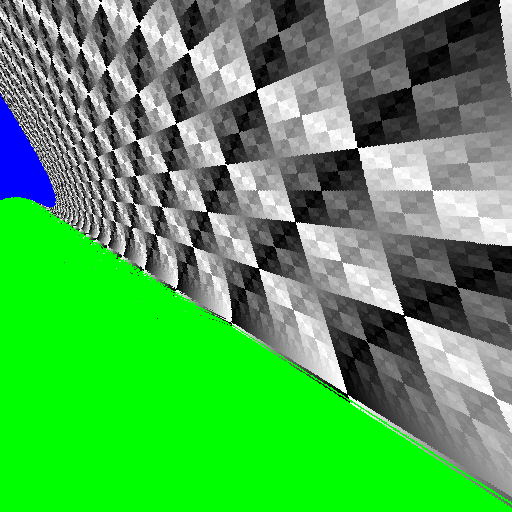
\includegraphics[width=\columnwidth]{sqrt.png}

\section*{Raycasting}

\subsection*{Why raycasting is necessary}

Computer images are (normally, and right now you can pretend that they are always) made of pixels - a 2d lattice of points and associated colors for screen rendering.  If you zoom really far into an image, it gets blurry because the pixels are so sparse, and the computer doesn't have much to work with.

A lot of rendering today is done by raycasting.  In raycasting, every pixel on the image that is being generated is assigned a vector.  The top left pixel of the image may correspond to a ray that goes in front, above, and to the left of the camera.  Each ray is then tested for intersection with the environment - whether or not it hits something, or where it ends up landing.  Depending on the result (hit/miss, near/far), the pixel corresponding to the ray can be filled in.

\subsection*{Ray tracing}

One technique for raycasting is called ray tracing.  Ray tracing involves mathematically determining the intersections between a line and a surface.  This can be a complicated thing for even simple cases.  To graph $z=e^x$, you would have to solve an intersection between a line and $e^x$.  The Lambert W function exists, but I did not believe (and still do not believe) that I could write a computer program that could automatically do algebra in an efficient manner.

\subsection*{Ray marching}

Another technique for raycasting is called ray marching.  In ray marching, the goal is to gradually move a point along the ray, until the distance between the point and the enviroment surface is 0.  This is where distance functions come in.  If you have a function that tells you the distance to the nearest point on the surface (or at least approximates it), then you know how far along you can move the point before there's a chance that you've moved it too far.

If the distance to the environment surface approaches 0, then my program assumes that the ray hits, and color is a greyscale color which corresponds to the $x$ and $y$ values.  If the distance grows very large, or the program has moved the point along the ray too many times without hitting something, my program assumes that the ray does not hit, and color it blue.  If the distance is undefined (which could happen outside of the domain of the function), then my program colors it green.

\section*{Cube map}

I made an intermediate stage between casting the rays and displaying them.

With this technique, the program puts an axis-aligned cube around the camera.  It then draws a texture on each of the faces of the cube.  Once it has the cube, it can look up for each pixel in the image (and a latitude and longitude for the direction the camera is pointing) what color the pixel should be.

Painting the cube takes about 6 times as long as painting the screen directly, but I expect the position of the camera to change infrequently due to the nature of camera movement in the program.  The camera can rotate any which way, and the program won't have to make a new cube map until the camera's position changes!

A technology (WebGL/OpenGL) does exist that could make drawing the cube map to the screen even faster so it isn't slowed down on devices slower than my laptop, but I've tried it a couple of times outside of this project and could not figure it out.  I did not feel confident using it for this project.

\section*{Distance estimator}

The original proposal was to use signed distance functions, but signed distance functions turned into signed distance estimators (because not all signed distance functions are solvable), and signed distance estimators turned into distance estimators because a good-ish unsigned distance estimator was easier to implement.  This distance estimator this program uses was artifically modified to be signed in order to handle different cases easier.

In order to get a distance estimate, the program measures the distance to a cone.  The pointy point on this cone has the same $x$ and $y$ of the sample point, but its $z$ is $f(x,y)$ - it lies on the surface.  Its slope is equal to $\pm\nabla f(x,y)$.  The large problem in using them is that they may be inaccruate, especially when the derivatives change rapidly, because this cone relies on the maximum gradient being constant.

I had also tried a paraboloid (like the next step after the cone of some Taylor series with 2 input variables), but that was getting complicated.  The distance function for a parabola contains trigonometric and power functions, which are computationally slow compared to multiplication and addition, and such a function for a paraboloid could be much worse, so I decided to stop bothering with it.

\section*{Function input}

This program uses RPN (postfix) function input.

This part of the program works by storing a constant array of terms and stack of computer instructions to work with.  'x', 'y', and any number and a couple of constants in the list of terms are directions to put that thing on the stack.  The term '2pi' will put the computer instruction '(2 * Math.PI)' on the stack.  Functions in the list of terms will do operations on the stack - if the last two stack items are 'x' and 'y', and the newest term is '+', those two items on the stack will turn into '(x+y)'.  The 'x' and 'y' will be removed from the stack, and the computer instruction '(x+y)' will be put on the stack.

After these operations, there should only be one big computer instruction left on the stack (like '((x+y)*5)').  This is the code that the web browser can run.

I chose to leave running the code to the web browser because if I ran the code myself, it would likely be slower due to the interpretation that the program would have to do.

\section*{Remaining bugs}

There is a bug where the ray march gives unexpected results for rendering and teleporting for functions without an $\R^2$ domain.  Cause is unknown.

\section*{Bibliography}

David J. Peterson.  ``The 2019 Smiley Award Winner: Fith,'' \url{https://dedalvs.com/smileys/2019.html}.  Accessed 29 November 2021.

Claude Leibovici et al.  ``Intersection of an exponential function and a line'', \url{https://math.stackexchange.com/questions/2632170/}.  Accessed 29 November 2021.

``Cube mapping,'' \url{https://en.wikipedia.org/wiki/Cube_mapping}.  Accessed 29 November 2021.

Inigo Quilez.  ``2D distance functions,'' \url{https://iquilezles.org/www/articles/distfunctions2d/distfunctions2d.htm}.  Accessed 29 November 2021.

\end{document}
